\chapter{Taurus Molecular Cloud}
\label{sec:Taurus}

\section{Structure and Properties}
Taurus lies at the boundary of two expanding interstellar structures, the Local Bubble and the Perseus-Taurus shell. \citet{Soler2023} argue that the converging flows driven by both structures triggered its formation. The Orion-Eridanus superbubble also lies in the broader vicinity of Taurus \cite{Ochsendorf2015}, another large, low-density and dust-poor cavity in the local ISM named after the Orion star forming region, which is the assumed source. The proximity to all these large structures (interessante entstehungsmöglichkeiten erwähnen)

An interactive 3D map of the solar neighborhood with the most prominent star-forming regions on the surface of the Local Bubble, as well as the 3D shapes and motions of their young stellar clusters, presented by \citet{Zucker2022} can be viewed at (\href{https://faun.rc.fas.harvard.edu/czucker/Paper_Figures/Interactive_Figure1.html}{interactive}).
A more detailed model, showing the Local Bubble as a system of several shells that are open to the Galactic halo rather than a single fully enclosed shell, was presented by \citet{Oneill2024} and is available at (\href{https://theo-oneill.github.io/localbubble/plots/bubble_enviro.html}{interactive}); a snapshot of this model is shown in Figure~\ref{fig:Local_Bubble}.

\begin{figure}[h!]
    \centering
    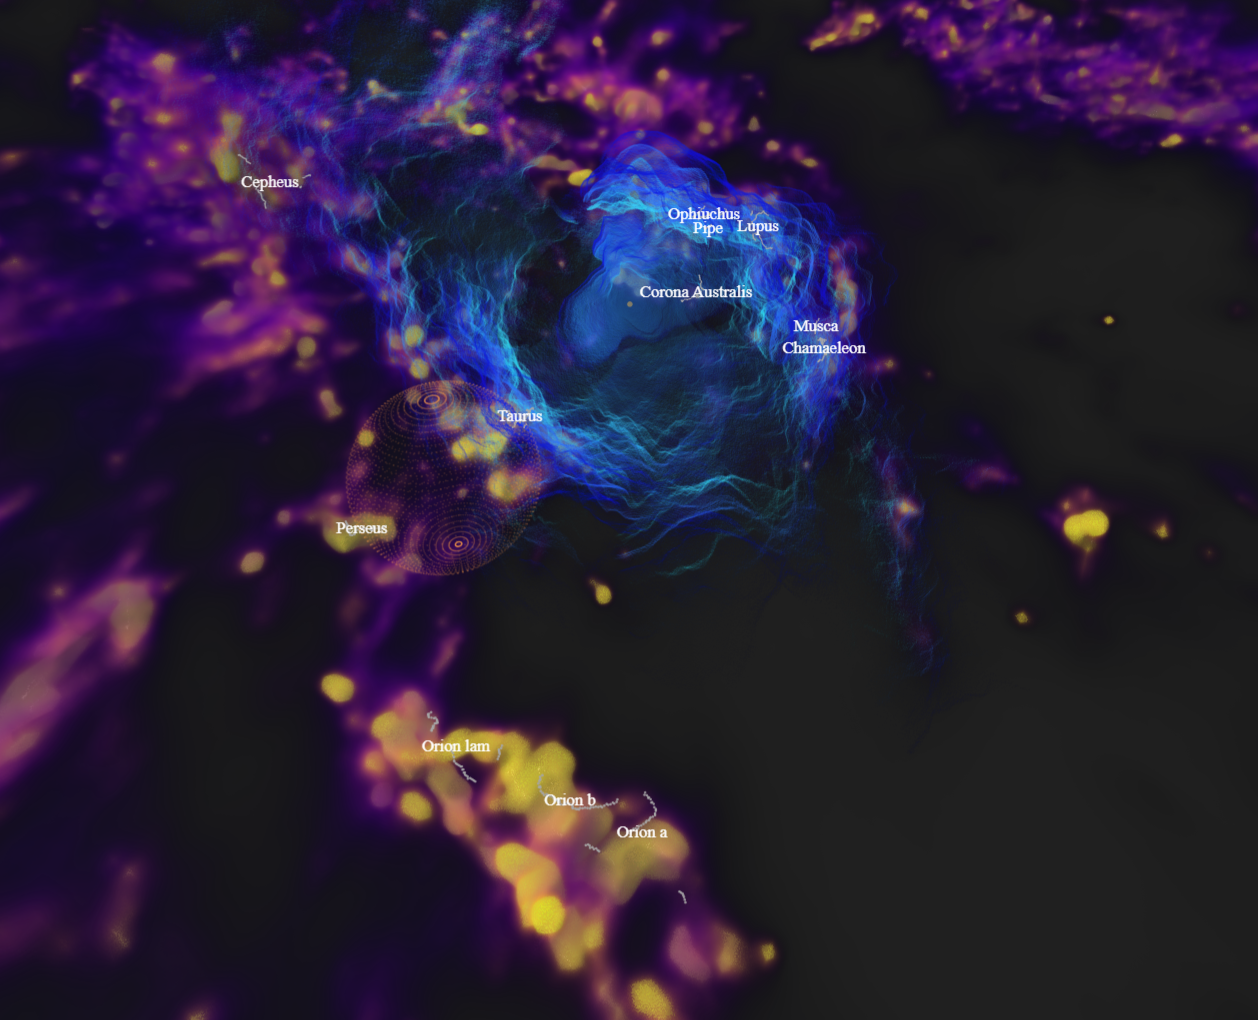
\includegraphics[width=0.8\linewidth]{figures/Local_Bubble.PNG}
    \caption{Snapshot of the interactive three-dimensional dust map of the solar neighborhood from \citet{Oneill2024}, showing prominent nearby molecular clouds and star-forming regions around the low-density cavity of the Local Bubble; Taurus lies along its edge, adjacent to Perseus.}
    \label{fig:Local_Bubble}
\end{figure}

The TMC is one of the most intensively studied low-mass star-forming regions in the Milky Way. It spans a total of about $15 \times 15$~degrees on the sky and lies at a distance of approximately 140~parsecs from Earth, although significant depth effects are present along the line of sight, with substructures spanning distances from roughly 128~pc to nearly 200~pc. The complex hosts a few hundred YSOs that are not randomly distributed but instead clustered into small groups \cite{Galli2019}.


\begin{figure}[h!]
    \centering
    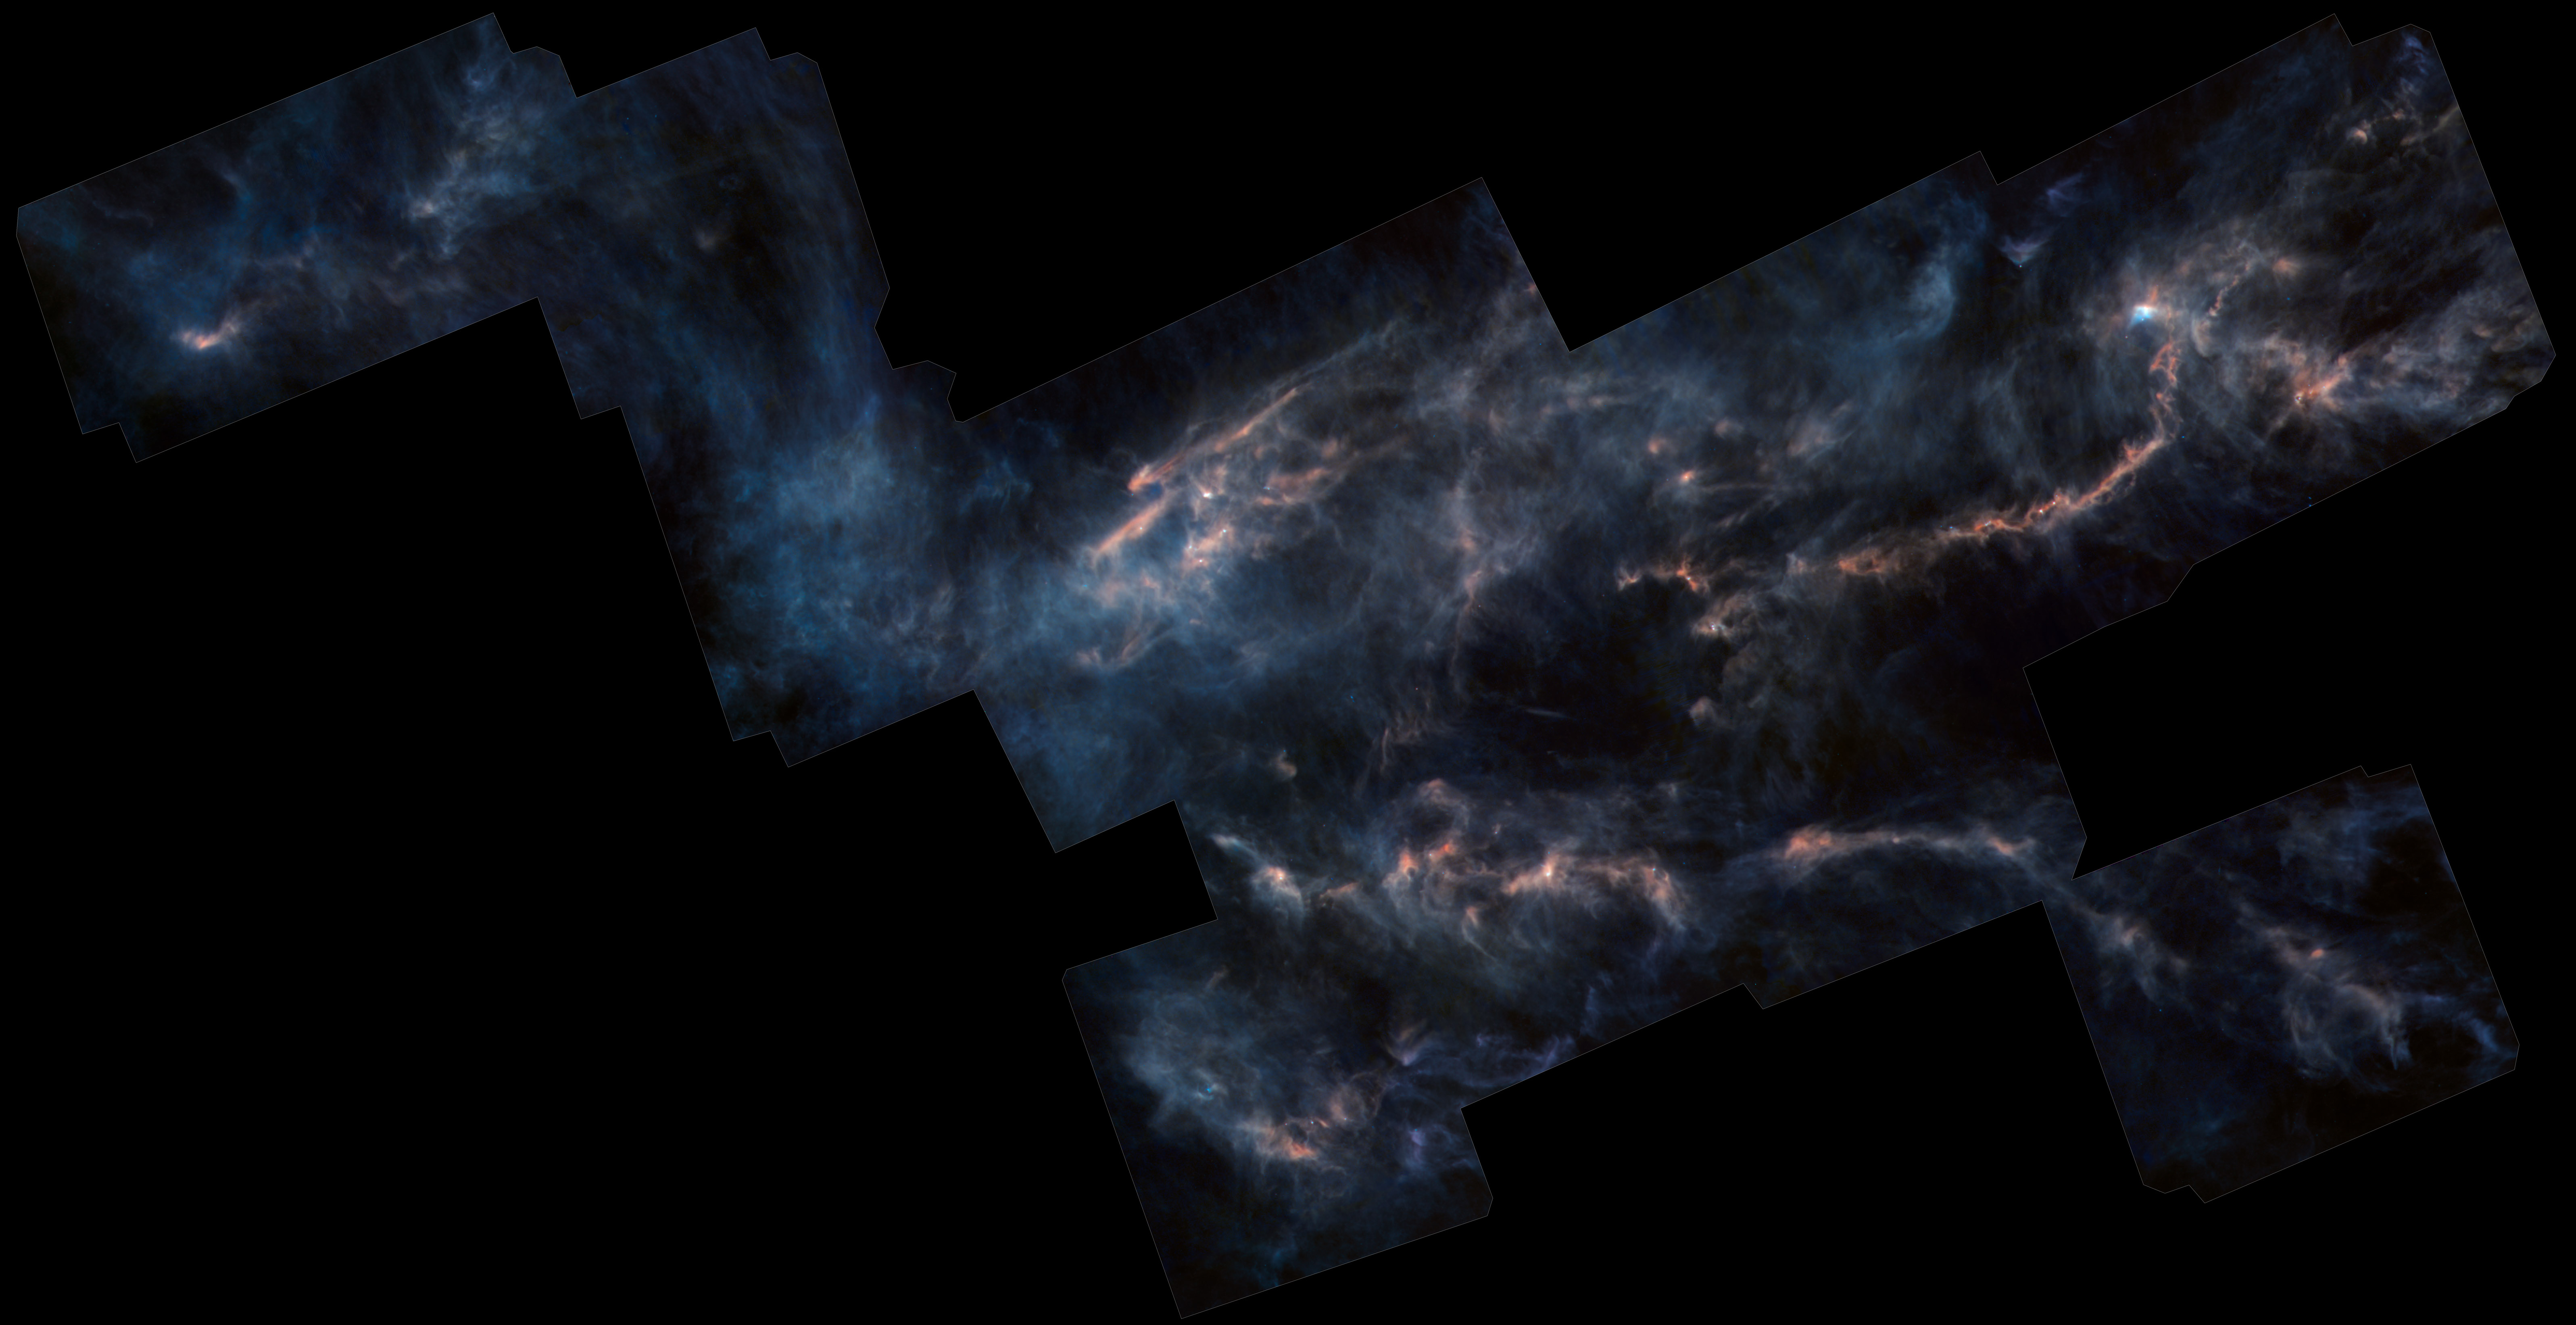
\includegraphics[width=\linewidth]{figures/Taurus_sky_view.jpg}
    \caption{"This mosaic combines several observations of the Taurus Molecular Cloud performed by ESA’s Herschel observatory." \cite{ESA2017Taurus}}
    \label{fig:Taurus_sky}
\end{figure}

The most recent census, based on Gaia~DR3, revised the total membership to 532 adopted members distributed across 13 kinematic groups, most with median ages of $1$--$3$~Myr, while neighbouring associations have ages ranging from 13 to 56 Myr. Samples of older stars ($\geq10$ Myr) in the vicinity of Taurus were proposed to also be associated with the cloud but where not included in the catalog because of inconsistent kinematics compared to Taurus \cite{Luhman2023}.

\section{Kinematics}
The kinematics of Taurus have been the subject of several studies, enabled by increasingly precise astrometric data. An early investigation by \citet{Bertout2006} used proper motions supplemented by radial velocities to identify 94 probable members of the Taurus-Auriga moving group and to derive individual kinematic parallaxes, yielding a mean distance of 140~pc and a spatial velocity dispersion of approximately $6~\mathrm{km\,s^{-1}}$ across the association.

A more complete and precise picture was established by \citet{Galli2019}, who combined Gaia~DR2 astrometry with VLBI measurements from the GOBELINS project for a sample of 415 stars. Applying a hierarchical clustering algorithm, they identified 21 clusters, of which 13 could be associated with distinct molecular clouds, and derived their distances and spatial velocities. They found inter-cloud relative motions ranging from about 1 to $5~\mathrm{km\,s^{-1}}$, a median inter-cloud separation of 25~pc, and a one-dimensional velocity dispersion of the full sample on the order of $2~\mathrm{km\,s^{-1}}$. No significant expansion or contraction pattern was detected for the complex as a whole, although evidence for a potential global rotation was reported. The stellar velocities were furthermore found to closely match those of the underlying $^{13}$CO molecular gas, confirming a tight dynamical coupling between the stars and the gas.

This picture was extended by \citet{Soler2023}, who combined 3D dust reconstruction with CO gas emission and neutral hydrogen observations to study the large-scale cloud dynamics. Their analysis revealed a velocity gradient across the cloud consistent with external compression, in line with the bubble geometry described above. Despite this progress, the internal kinematics of Taurus remain incompletely characterized, in part because radial velocity measurements are available for only a subset of its members. This motivates a complementary approach that uses the full available data of Gaia proper motions to reconstruct a continuous 3D velocity field across the complex, as pursued in this thesis.